\documentclass[journal=nalefd,manuscript=letter]{achemso}
\setkeys{acs}{articletitle=true}
\usepackage{graphicx}
\usepackage{amsmath}
\usepackage{amssymb}
\usepackage{subfigure}
\usepackage{xr}
%%This is for adding a footer with the time of the compilation of the file.
%%Useful for versioning of printed copies.
%\usepackage{datetime}
%\usepackage{fancyhdr}
%\fancyfoot[L]{\fontsize{8}{12} \selectfont \today $\,$ \currenttime}
%\pagestyle{fancy}
%%%%%%%%%%%%%%%%%%%%%%%%%%%%%%%%%%%%%%%%%%%%%%%%%%%%%%%%%%%%%%%%%%%%%
%%%%%%%%%%%%%%%%%%%%%%%%%%%%%%%%%%%%%%%%%%%%%%%%%%%%%%%%%%%%%%%%%%%%%

%\usepackage[version=3]{mhchem} Formula subscripts using \ce{}
\usepackage[T1]{fontenc} %      Use modern font encodings
\externaldocument{anti_stokes}
\renewcommand{\thefigure}{S\arabic{figure}}

\newcommand{\K}{\ensuremath{\,\textrm{K}}}
\newcommand{\nm}{\ensuremath{\,\textrm{nm}}}
\newcommand{\mm}{\ensuremath{\,\textrm{mm}}}
\newcommand{\um}{\ensuremath{\,\mu\textrm{m}}}
\newcommand{\m}{\ensuremath{\,\textrm{m}}}
\newcommand{\eV}{\ensuremath{\,\textrm{eV}}}
\newcommand{\uM}{\ensuremath{\,\mu\textrm{M}}}
\newcommand{\uW}{\ensuremath{\,\mu\textrm{W}}}
\newcommand{\mW}{\ensuremath{\,\textrm{mW}}}
\newcommand{\W}{\ensuremath{\,\textrm{W}}}
\newcommand{\pM}{\ensuremath{\,\textrm{pM}}}
\newcommand{\meV}{\ensuremath{\,\textrm{meV}}}
\newcommand{\pwr}{\ensuremath{\,\textrm{kW/cm}^2}}
\newcommand{\fs}{\ensuremath{\,\textrm{fs}}}
\newcommand{\ps}{\ensuremath{\,\textrm{ps}}}
\newcommand{\CPS}{\ensuremath{\,\textrm{CPS}}}
\newcommand{\kCPS}{\ensuremath{\,\textrm{kCPS}}}
\newcommand{\atto}{\ensuremath{\textrm{ATTO}\,647\textrm{N}}}
\newcommand{\degree}{\ensuremath{\,^o\textrm{C}}}

\author{Aquiles Carattino}
\affiliation[Leiden]
{Huygens-Kamerlingh Onnes Lab, 2300RA Leiden, The Netherlands}
\author{Mart\'in Caldarola}
\affiliation[Leiden]
{Huygens-Kamerlingh Onnes Lab, 2300RA Leiden, The Netherlands}
\author{Michel Orrit}
\email{orrit@physics.leidenuniv.nl}
\affiliation[Leiden]
{Huygens-Kamerlingh Onnes Lab, 2300RA Leiden, The Netherlands}

\title{Gold nanoparticles as absolute nano-thermometers. \\
Supporting information}

\keywords{Gold nanorods, Plasmon, Anti-Stokes, Sensing, Temperature}

\begin{document}

\maketitle



\section{Anti-Stokes emission form gold nanorods}\label{sec:AS}

We model the photoluminescence generation in gold nanorods with successive 
steps taking place between absorption of light and re-emission of luminescence\cite{Carattino2016a}. 
Figure \ref{fig:anti-Stokes-process} shows the energy-momentum representation
of the photoluminescence processes in gold nanorods. 
After excitation with monocrhomatic light of energy $\hbar \omega_L$, 
a collective oscillation of electrons is generated, i.e. a surface plasmon (SPR). 
Once the plasmon coherence is lost (dephasing time $\sim$fs), the state can be described as an
electron-hole pair. Then, different scenarios are possible: recombination 
without energy exchange, elastic recombination (leading to Rayleigh scattering) or 
recombination with energy exchange. In this case, three scenarios are possible: electron and hole may
recombine radiatively after one or more interactions with the thermal baths of
lattice phonons and charge carrier thermal excitations: i) if the energy
difference between electron and hole states is lower than the initial one after
excitation we obtain Stokes emission upon a radiative recombination; ii) if
electron and hole transiently increase their energy difference at the bath's
expense before recombining radiatively, we observe anti-Stokes emission; iii) if
electron and hole recombine non radiatively, their energy difference is
transferred to the baths and no photon is emitted. The latter process is the
most probable one, explaining the low yield of luminescence in gold ($\sim 10^{-6}$). 

\begin{figure}[htp] \centering
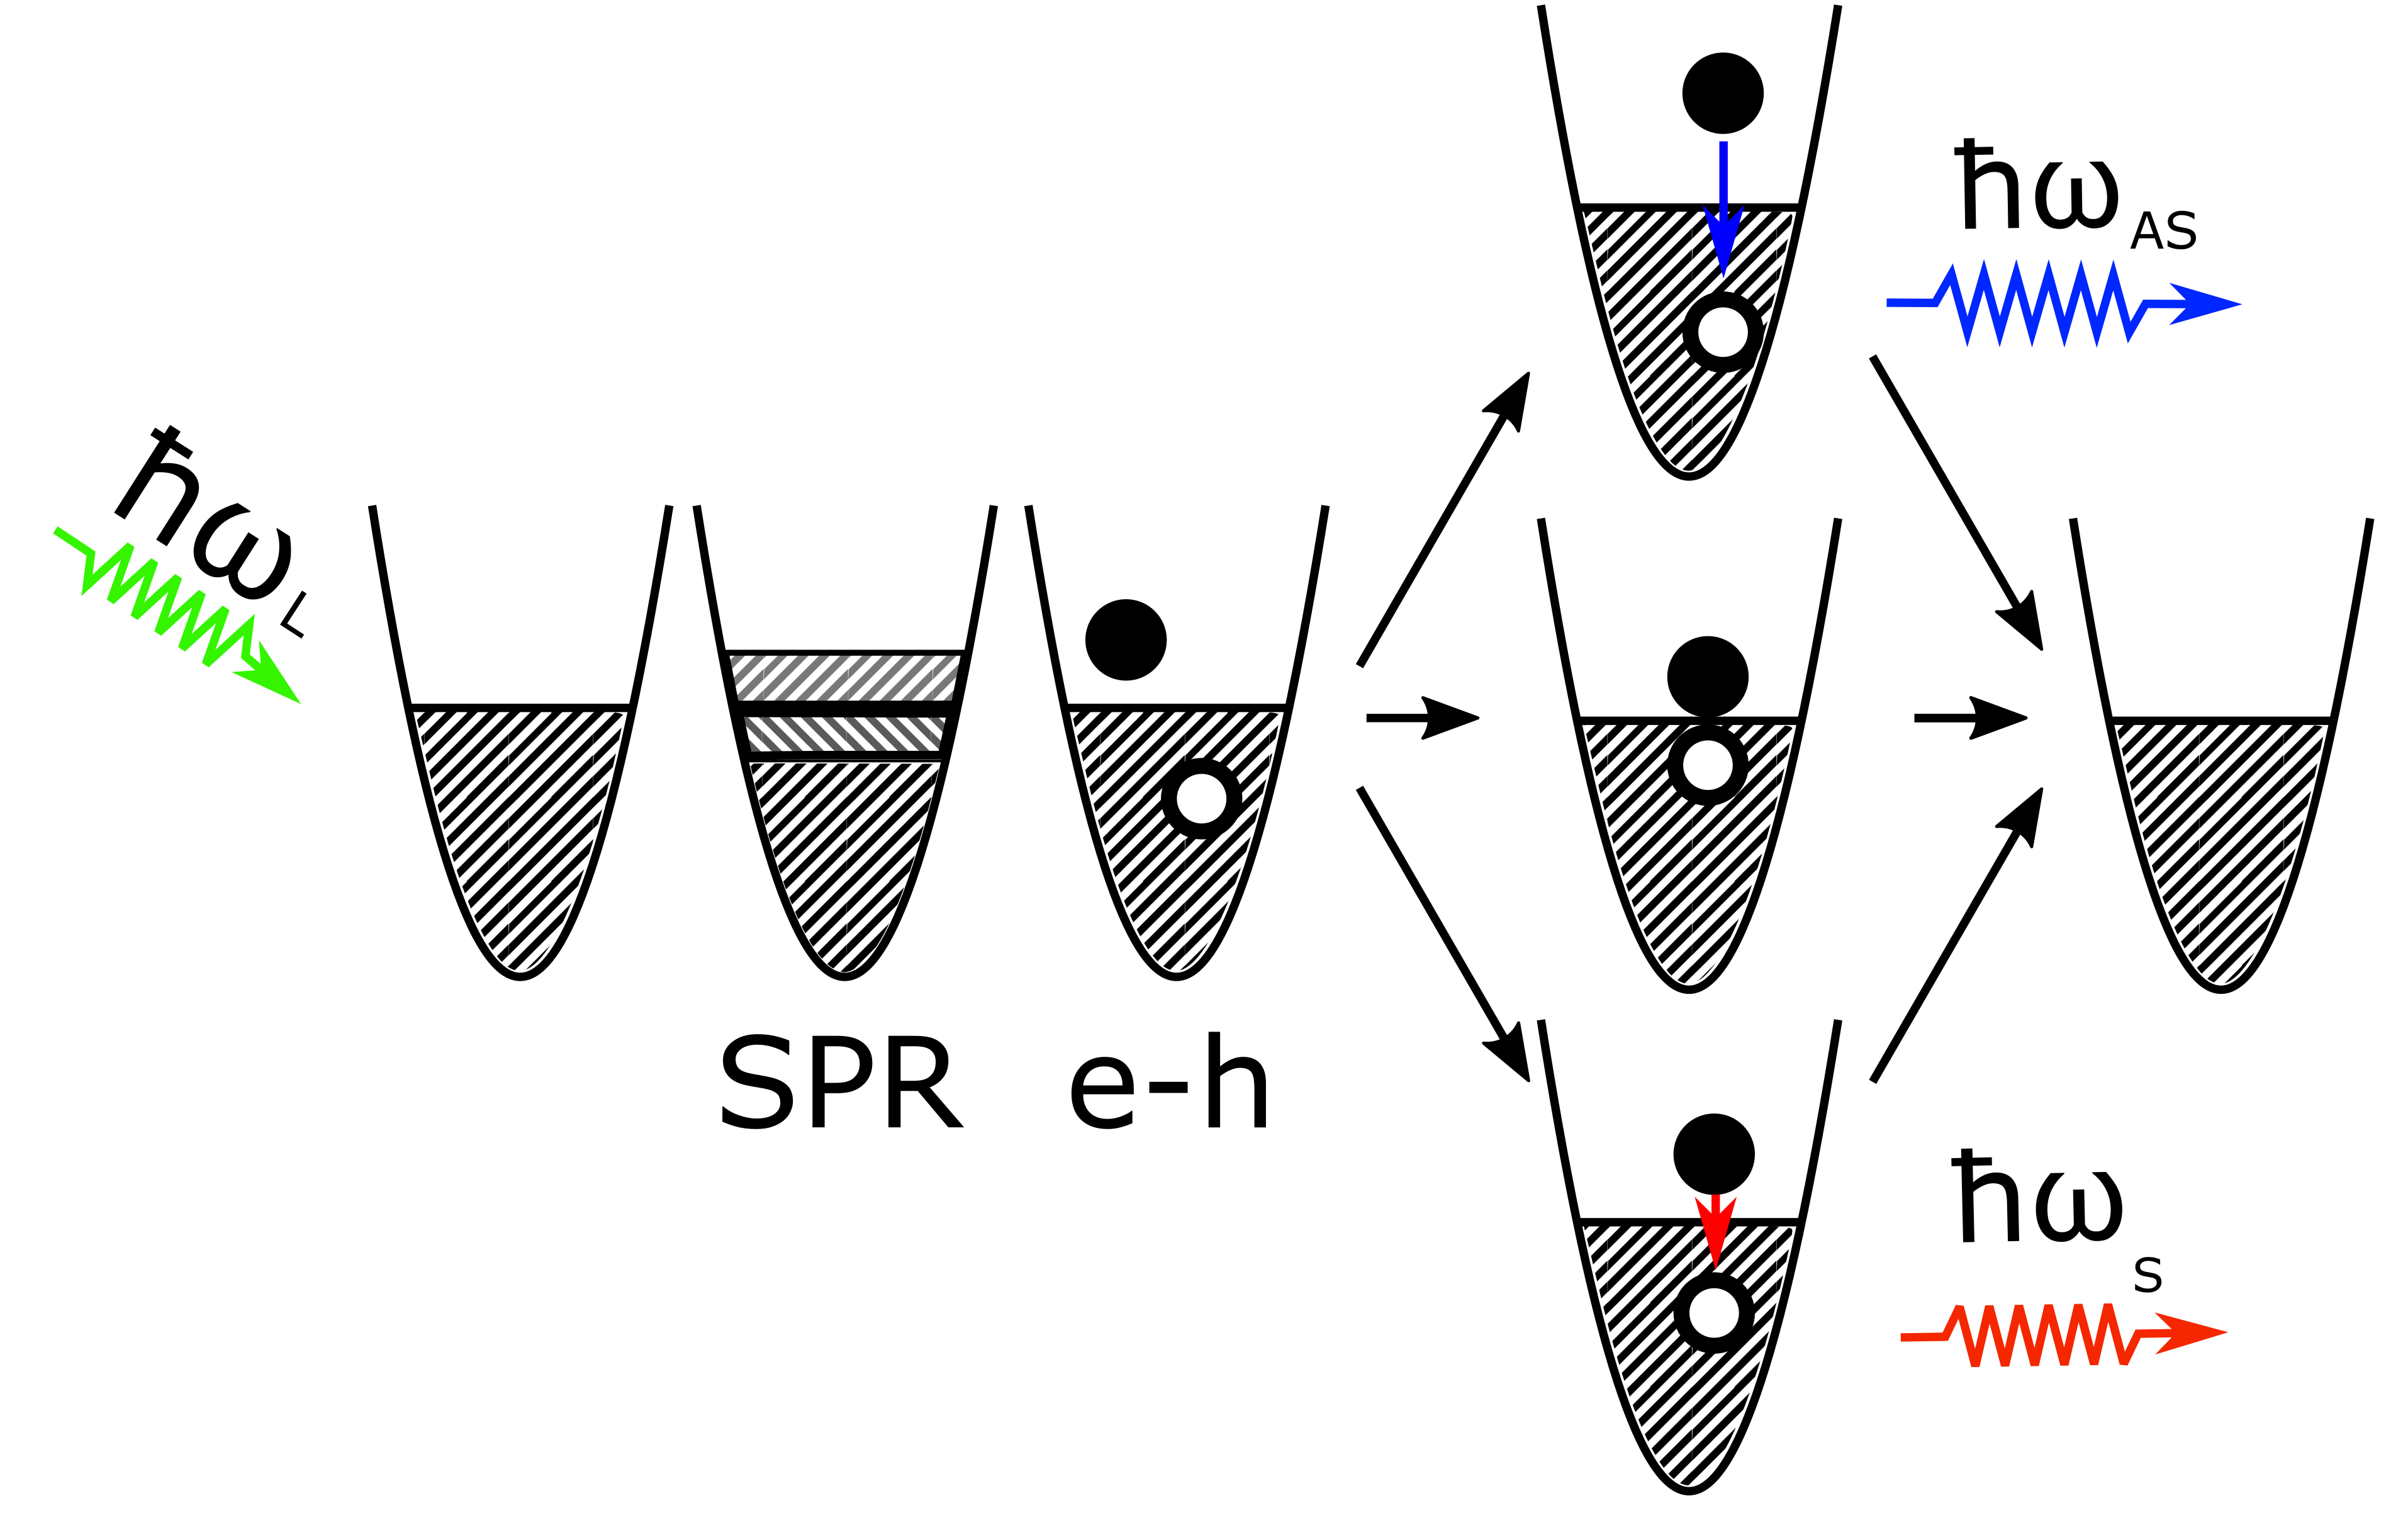
\includegraphics[width=0.5\textwidth]{Figures/Supplementary/01_AS_Scheme/luminescence_all_AS.png}
\caption{\textbf{Schematic representation of Stokes and Anti-Stokes luminescence process from a single gold nanorod.} 
Upon the excitation with resonant energy $\hbar \omega\textrm{L}$ a surface plasmon is created (SPR), which creates 
an electron-hole pair state (e-h). This pair can recombine non-radiatively (the most likely event) or radiatively
after iterating with the baths, leading to high energy (anti-Stokes) or low energy (Stokes) emission of a photon.}
	\label{fig:anti-Stokes-process}
\end{figure}


\section{Experimental setup}\label{sec:setup}

The experimental setup consisted on a home-made confocal microscope, schematically shown in figure
\ref{fig:setup}, similar to the one presented before \cite{Carattino2016a}. The microscope allows 
the detection of individual nanorods in the sample and the measurement of their photoluminescence spectra. 
We use continuous wave lasers at 532 nm or 633 nm to excite the transverse and longitudinal plasmon resonances, respectively. The  532 nm is a DPSS laser (CNI) and the 633 nm is a HeNe (Thorlabs). Both lasers are reflected at a 50/50 beam splitter that allows the simultaneous detection of the anti-Stokes and Stokes emission of the particles.

We employ an objective lens to focus the excitation beam into a diffraction-limited 
spot and we collect the emitted photoluminescence using the same objective in an epi-configuration. 
The 532 nm laser is focused down by our 60x NA1.4 objective to a waist of 228 nm, with a power of $200 \mu$W reaching the sample, leading to an intensity of $1.23$ mW$\mu$m$^{-2}$. 
For the HeNe laser, the maximum power used was $100$ $\mu$W which 
corresponds to $0.43$ mW$\mu$m$^{-2}$. This is equivalent to $1.37\times10^{15}$ photons s$^{-1}$ $\mu$m$^{-2}$, which leads to a fluence of $\approx 240$ photons$\mu$m$^{-2}$ in three minutes integration time used for the spectra acquisition. 
A confocal pinhole of 50 $\mu$m is placed between a pair of lenses with 10 cm focal length to reduce the unwanted background from the solvent above the nanorods. Then we could select between an APD or the spectrometer to perform a raster-scan image or an emission spectrum, respectively. We reject the laser light with appropriate notch filters.

Additionally, the temperature of the sample can be controlled with a special holder that allows 
water flow, a heater and a thermocouple to measure the temperature of the sample. For the experiments
done with this holder we employed a 60X objective with NA $0.9$ (Olympus) to avoid presence of a heat sink on the 
particle under study.

\begin{figure}[htp] \centering
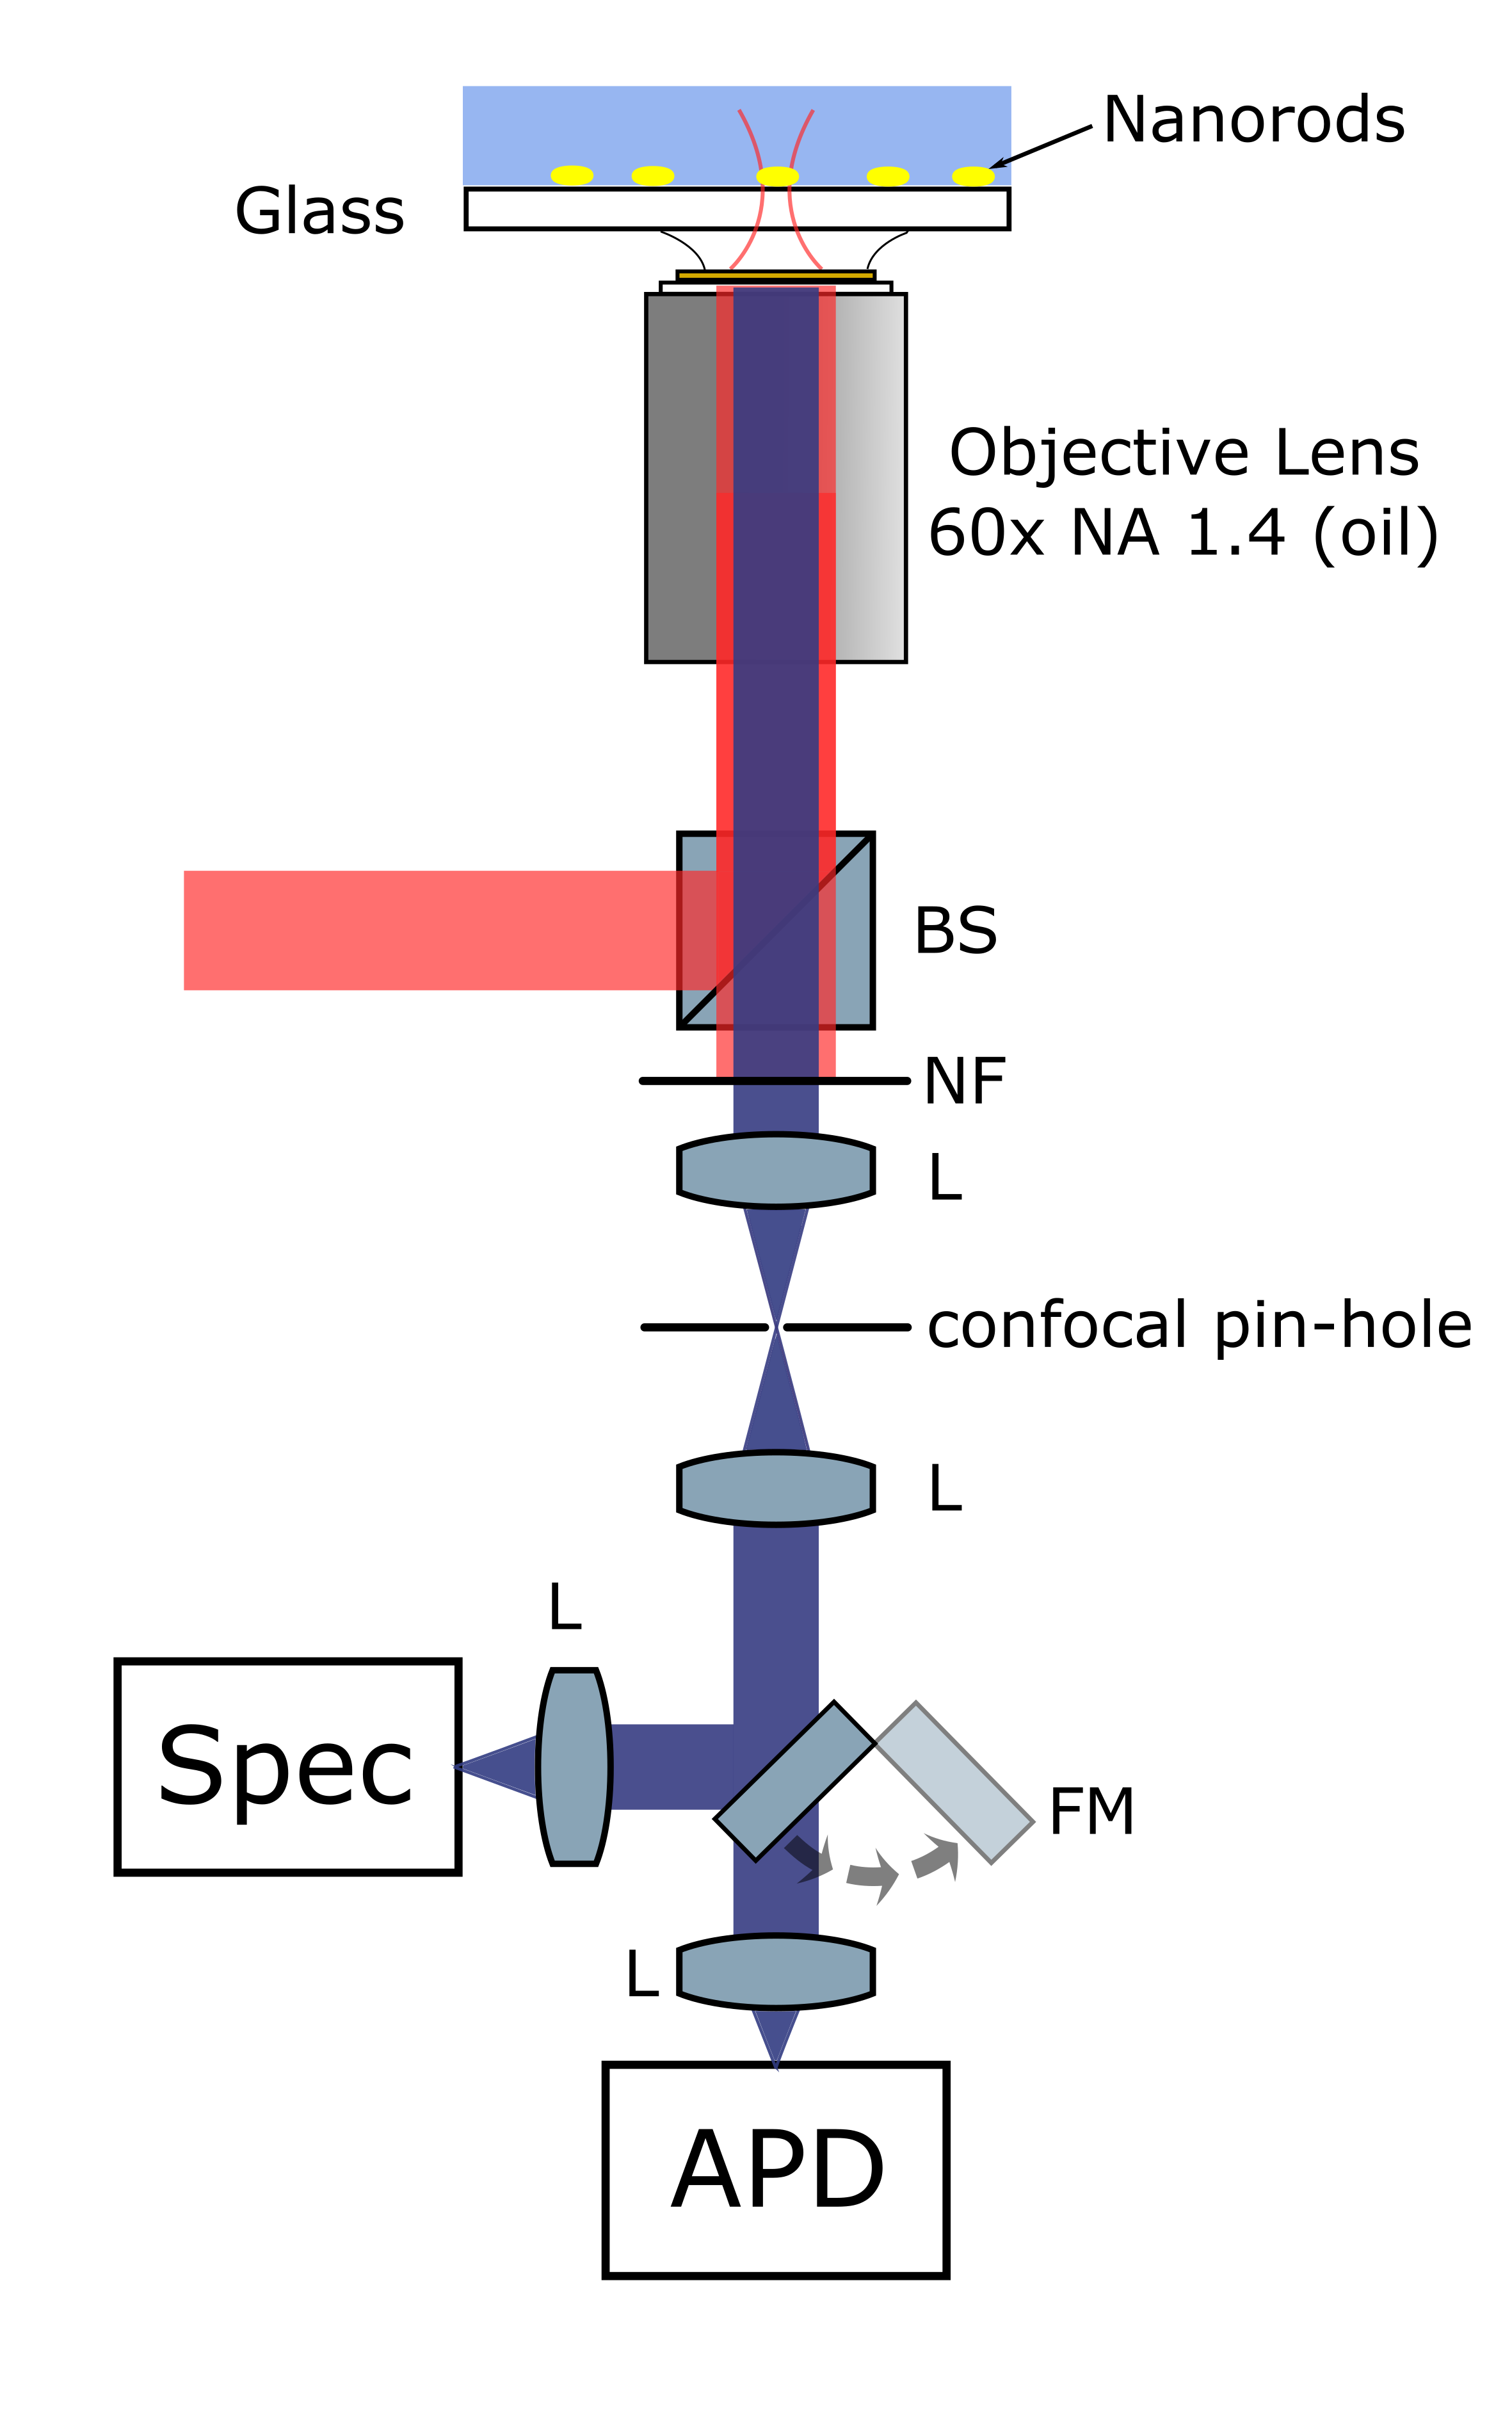
\includegraphics[width=0.5\textwidth]{Figures/Supplementary/02_Setup/setup.png}
\caption{\textbf{Scheme of the experimental setup.} The sample consists of individual gold nanorods immobilized on glass. BS: beam splitter. NF: notch filter to remove excitation light and detect Stokes and anti-Stokes photoluminescence. L: lens. FM: flip mirror. SPEC: spectrometer. APD: avalanche photodiode.}
	\label{fig:setup}
\end{figure}


\section{Gold nanorods sample characterization}

We synthesized gold nanorods using the seed-mediated growth method \cite{nikoobakht2003preparation} 
and characterized their size by performing TEM imaging on a drop-cast sample on a silicon substrate. 
Figure \ref{fg:nr-char} (a) shows the image where the cylindrical shape with spherical caps can be seen 
and the width is $23$ nm while the length is $50$ nm, 
leading to a mean aspect ratio of $2.17$. 
Naturally, there is some size dispersion due to the fabrication procedure, that leads to a broad bulk extinction 
spectra, shown in (b). The transverse plasmon resonance is located at $525$ nm while the more intense 
longitudinal plasmon resonance is at $630$ nm. We also show the wavelengths of the lasers used for 
our study as vertical lines. 

\begin{figure}[htp] \centering
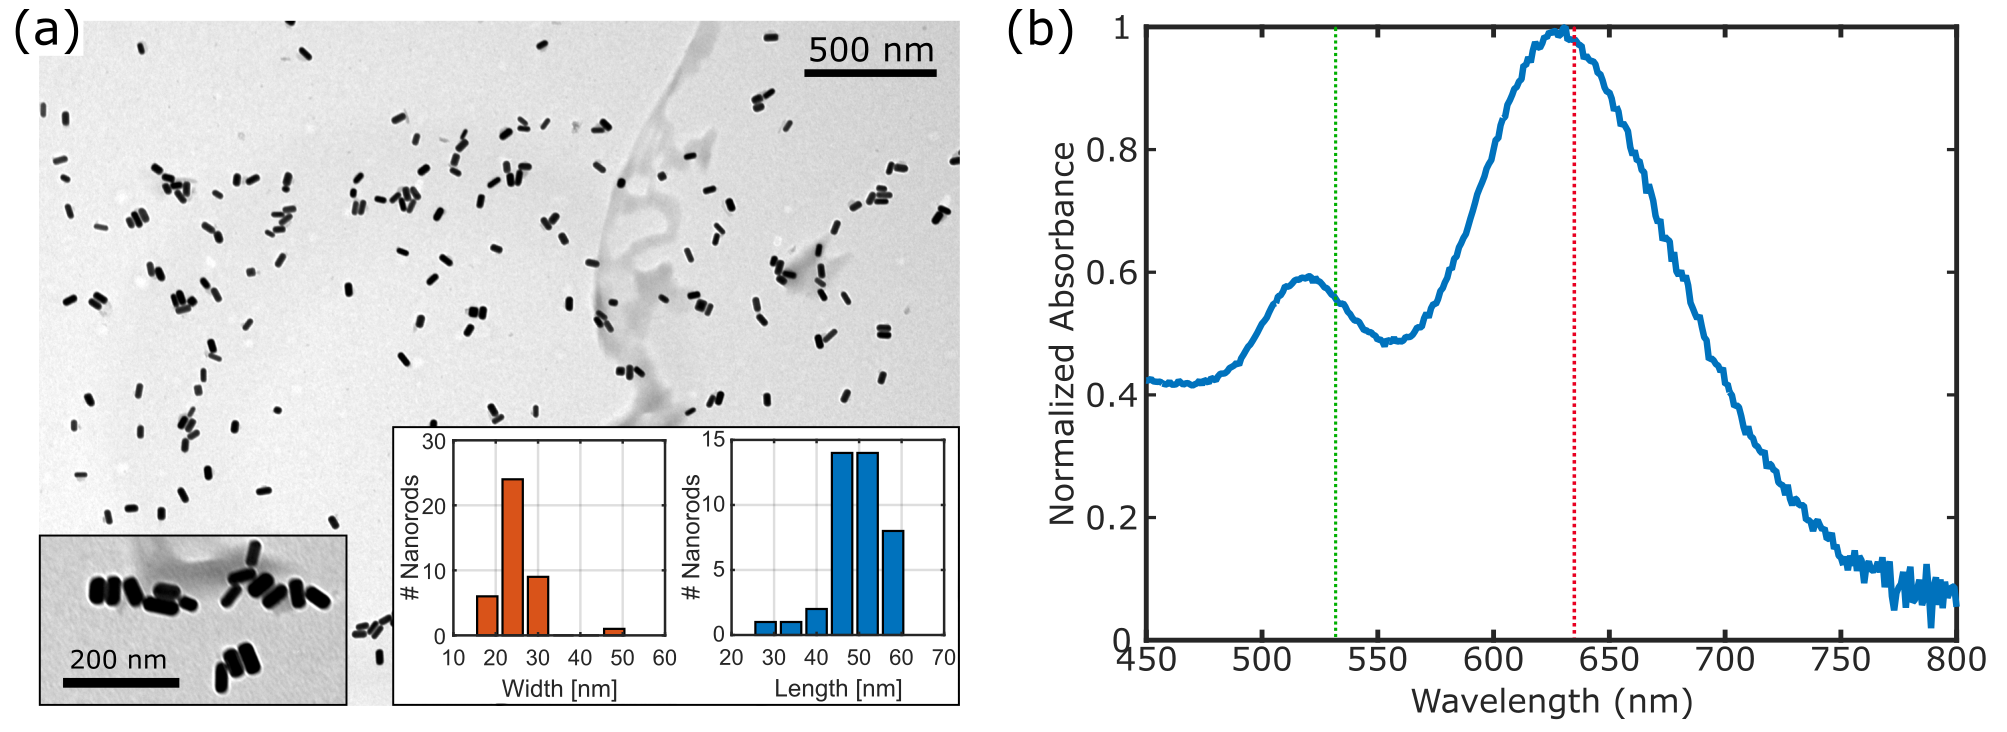
\includegraphics[width=0.8\textwidth]{Figures/Supplementary/07_GNRs_Characterization_TEM/GNRs_characterization.png}
\caption{\textbf{Gold nanorod characterization.} (a) TEM image of a dried drop of  the gold nanorods used in this study. The mean width is $23$ nm while the length is $50$. The inset shows higher magnification. (b) Bulk absorbance spectra of the gold nanorod sample showing the transverse (around $525$ nm) and the longitudinal (around $630$ nm) surface plasmon resonances. The dashed vertical lines show the two laser wavelengths used in this work.}
	\label{fg:nr-char}
\end{figure}


\section{Determination of the error in the temperature extraction}\label{sec:discussion_errors} 

The temperature extracted from the anti-Stokes spectrum depends on the initial fit of the plasmon resonance. The luminescence spectrum acquired with the $532\,\nm$ laser, shows an asymmetric shape due to a broadband contribution from gold added to the plasmonic emission. Therefore, the fitting of the SPR function ($I_\textrm{SPR}(E)$) of equation \ref{eqn:fitting} is not univocally determined; it will depend on the range of wavelengths selected for the fit. Therefore, the error of the method for temperature extraction can be estimated by studying the dependency of the final value with the intermediate parameters (i.e. the parameters of the lorentizan fit).

For the particle shown in Fig. \ref{fig:spectra_intensity}, changing the initial wavelength of the fit from $600\nm$ to $640\nm$ yields a significative difference in the obtained parameters of the lorentzian. Using the following expression for the $I_\textrm{SPR}$ function in $\eV$, 

\begin{equation*}
I_\textrm{SPR}(E) = \frac{P_1}{(E-P_2)^2+P_3}
\end{equation*}

We find that the values of $P_2$ lie between $1.940\eV$ and $1.955\eV$ and $P_3$ values between $8\cdot10^{-3}\eV^2$ and $8\cdot10^{-3}\eV^2$ for the different wavelength ranges. The value of $P_1$ is not relevant for the analyzis because it is only a normalization factor.

\begin{figure}[htp] \centering
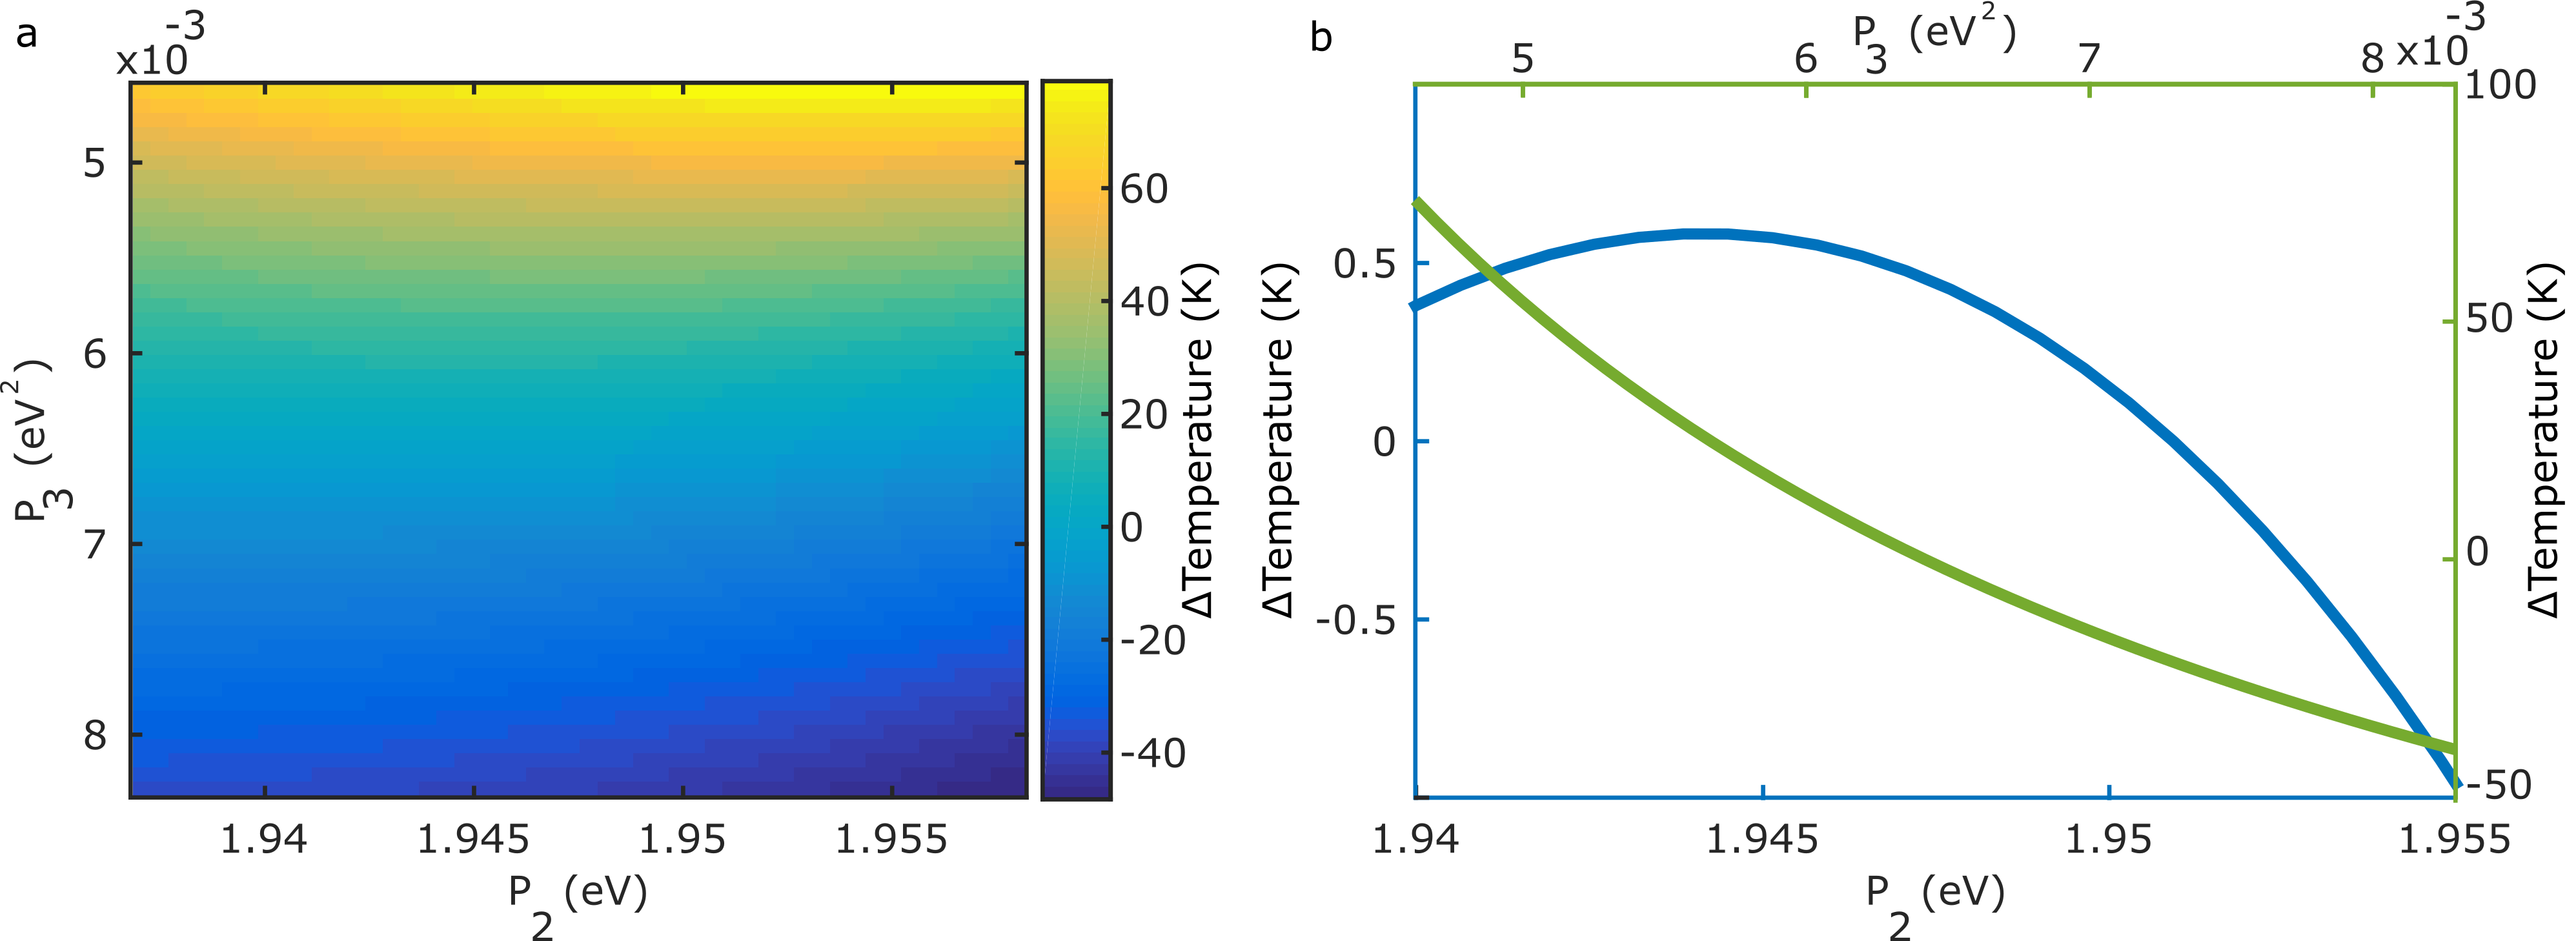
\includegraphics[width=0.90\textwidth]{Figures/Supplementary/05_Estimation_error/05_estimation_error.png}
\caption{Estimation of the error due to different fitting parameters of the plasmon spectrum. a) 2D grid of the difference in temperature obtained while varying both $P_2$ and $P_3$ parameters of the fit. b) Temperature dependence while keeping either $P_2$ or $P_3$ constant.}
	\label{fig:estimation-error}
\end{figure}

To study the impact that these different parameters have on the final result, we calculate the extracted temperature for all the combinations of $P_2$ and $P_3$, as is shown in Figure \ref{fig:estimation-error}.a. The color scale encodes the difference in temperature extracted compared to the value obtained with the parameters at the center of the range. Figure \ref{fig:estimation-error}.b shows two cross cuts of the temperature, while keeping either $P_2$ or $P_3$ constant.

In this example it is possible to note that the measured temperature is highly dependent on the fitted width of the plasmon spectrum ($P_3$) but barely dependent on its peak position ($P_2$). From the spectrum of the particle, it is possible to note that the wing of the plasmon coincides with the range of the anti-Stokes emission. Therefore, minute changes in the shape of the resonance will yield higher changes in the extracted temperature.

This assertion also implies that there should be particles in which the extracted temperature through the anti-Stokes fit wouldn't be too sensitive to the initial plasmon fit. To explore these possibilities, we calculated the anti-Stokes emission of different particles at $400\K$ by using equation \ref{eqn:fitting} and the results of ADDA calculations for the SPR function. From these data, we extracted the  temperature while varying the lorentzian parameters, exactly in the same way as what was done for the experimental results. We can therefore study the error in temperature for particles with different plasmonic resonances.

\begin{figure}[htp] \centering
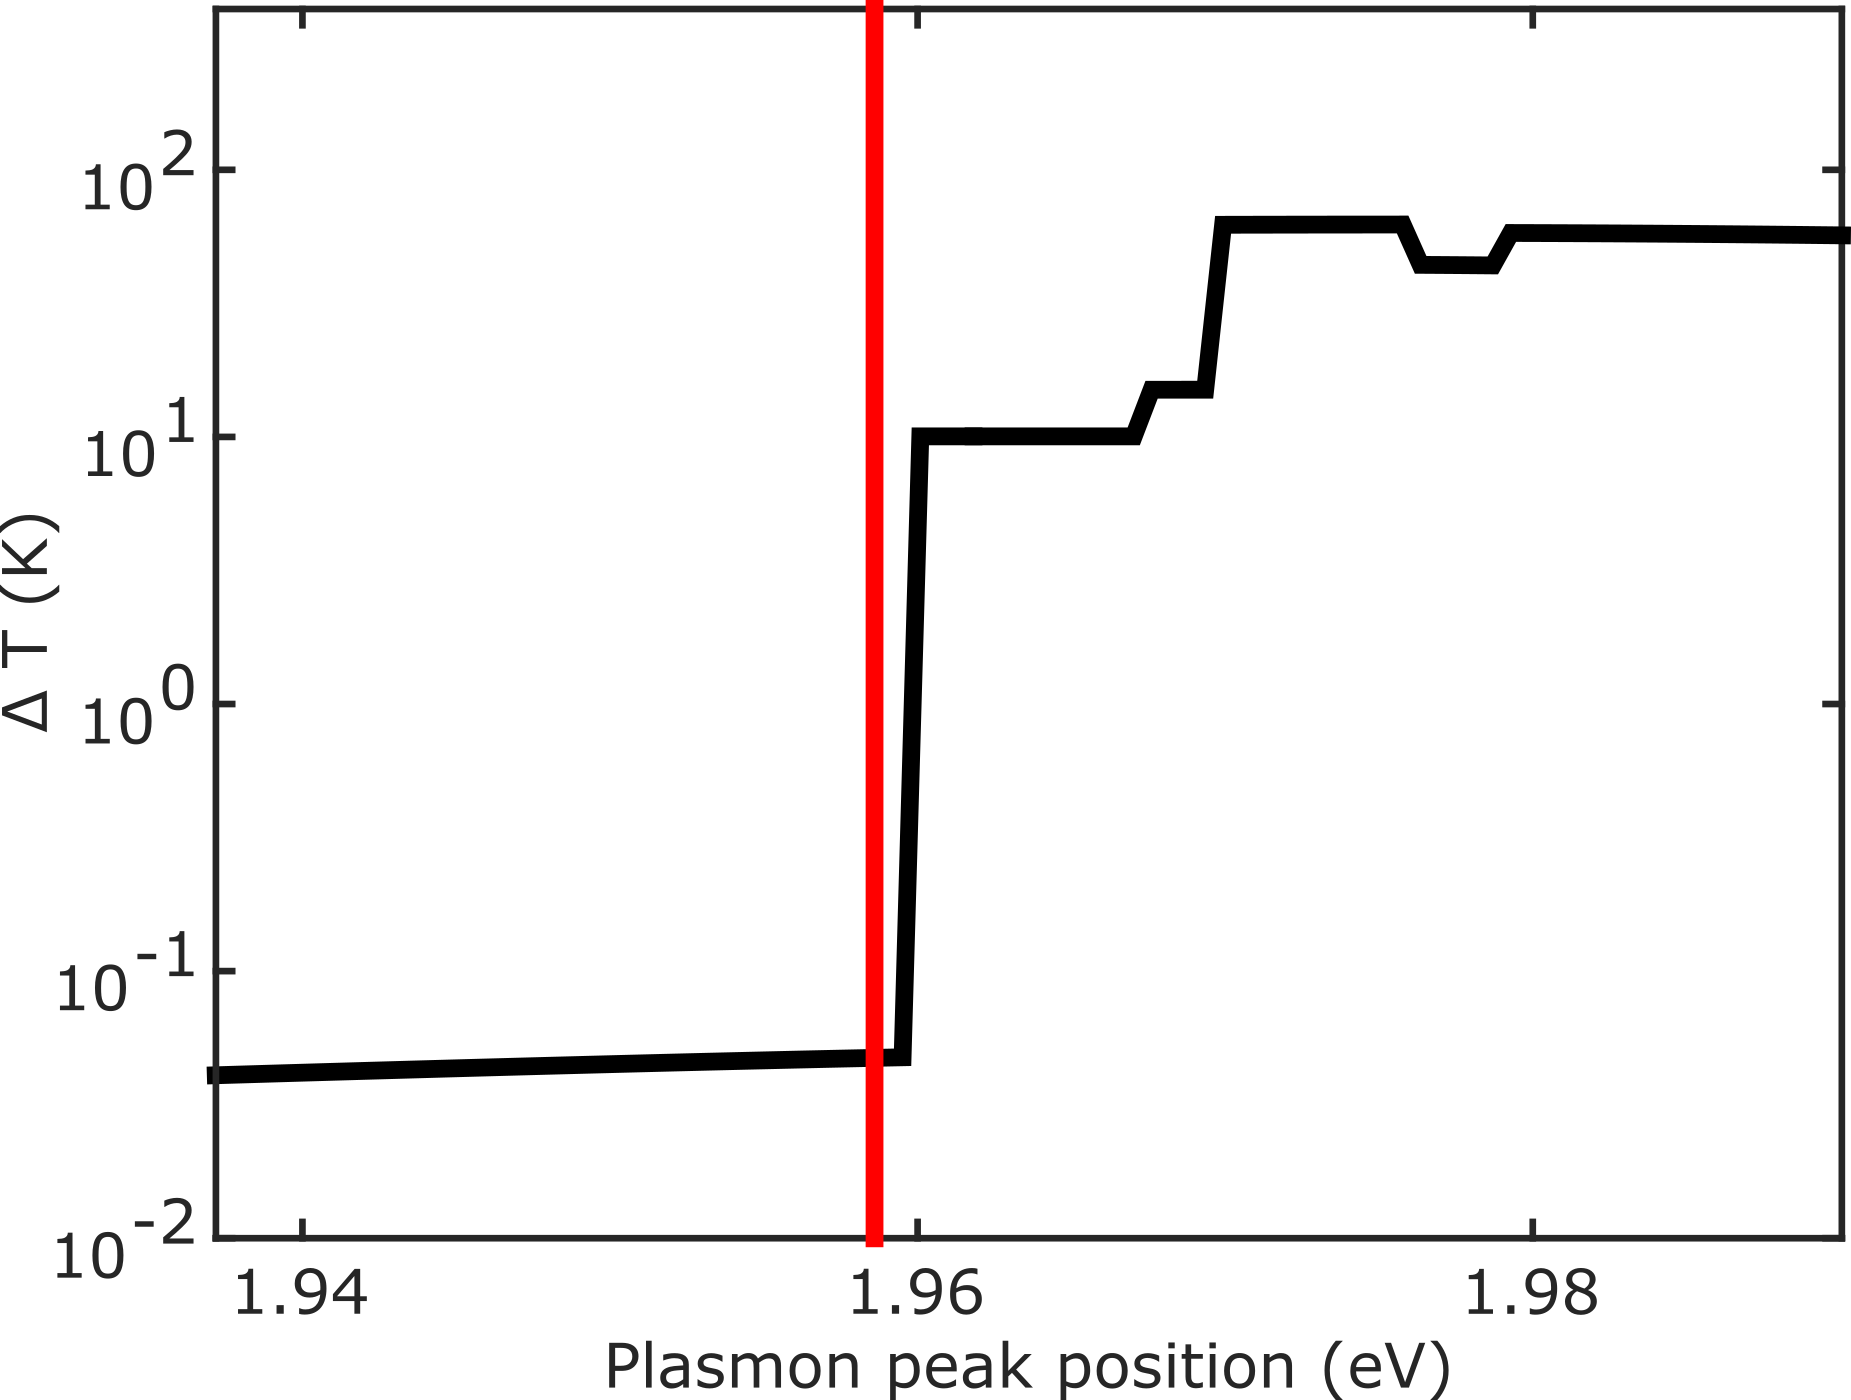
\includegraphics[width=0.45\textwidth]{Figures/Supplementary/06_Calculation_error/06_calculation_error.png}
\caption{Calculated error in the temperature extraction due to the uncertainty in the plasmon parameters as a function of the resonance position of the particle. Clearly, when exciting at the blue wing of the plasmon, the effect of these uncertainties is much lower.}
	\label{fig:calculated-error}
\end{figure}

Figure \ref{fig:calculated-error} shows the uncertainty in the extracted temperature as a function of the plasmon peak position. The uncertainty is defined as the difference between the maximum and the minimum extracted temperatures while varying $P_2$ by $10\%$ and $P_3$ by $30\%$. The vertical red line depicts the wavelength of the laser. It is remarkable that particles with a resonance red-shifted from the excitation laser present a much lower uncertanty in temperature as compared to particles with a resonance to the blue of the laser.

When the plasmon favors the anti-Stokes emission the correct modelling of the resonance is crucial for the extraction of temperatures. On the other hand, when the plasmon is red-shifted from the excitation, the induced error in the extracted temperature is much lower. However, the amount of collected light is another factor to keep into account. When the resonance is red-shifted from the laser, the anti-Stokes emission is much weaker and therefore accumulating enough photons in the spectrometer requires longer acquisition times. 

\section{Luminescence power dependence}

\begin{figure}[htp] \centering
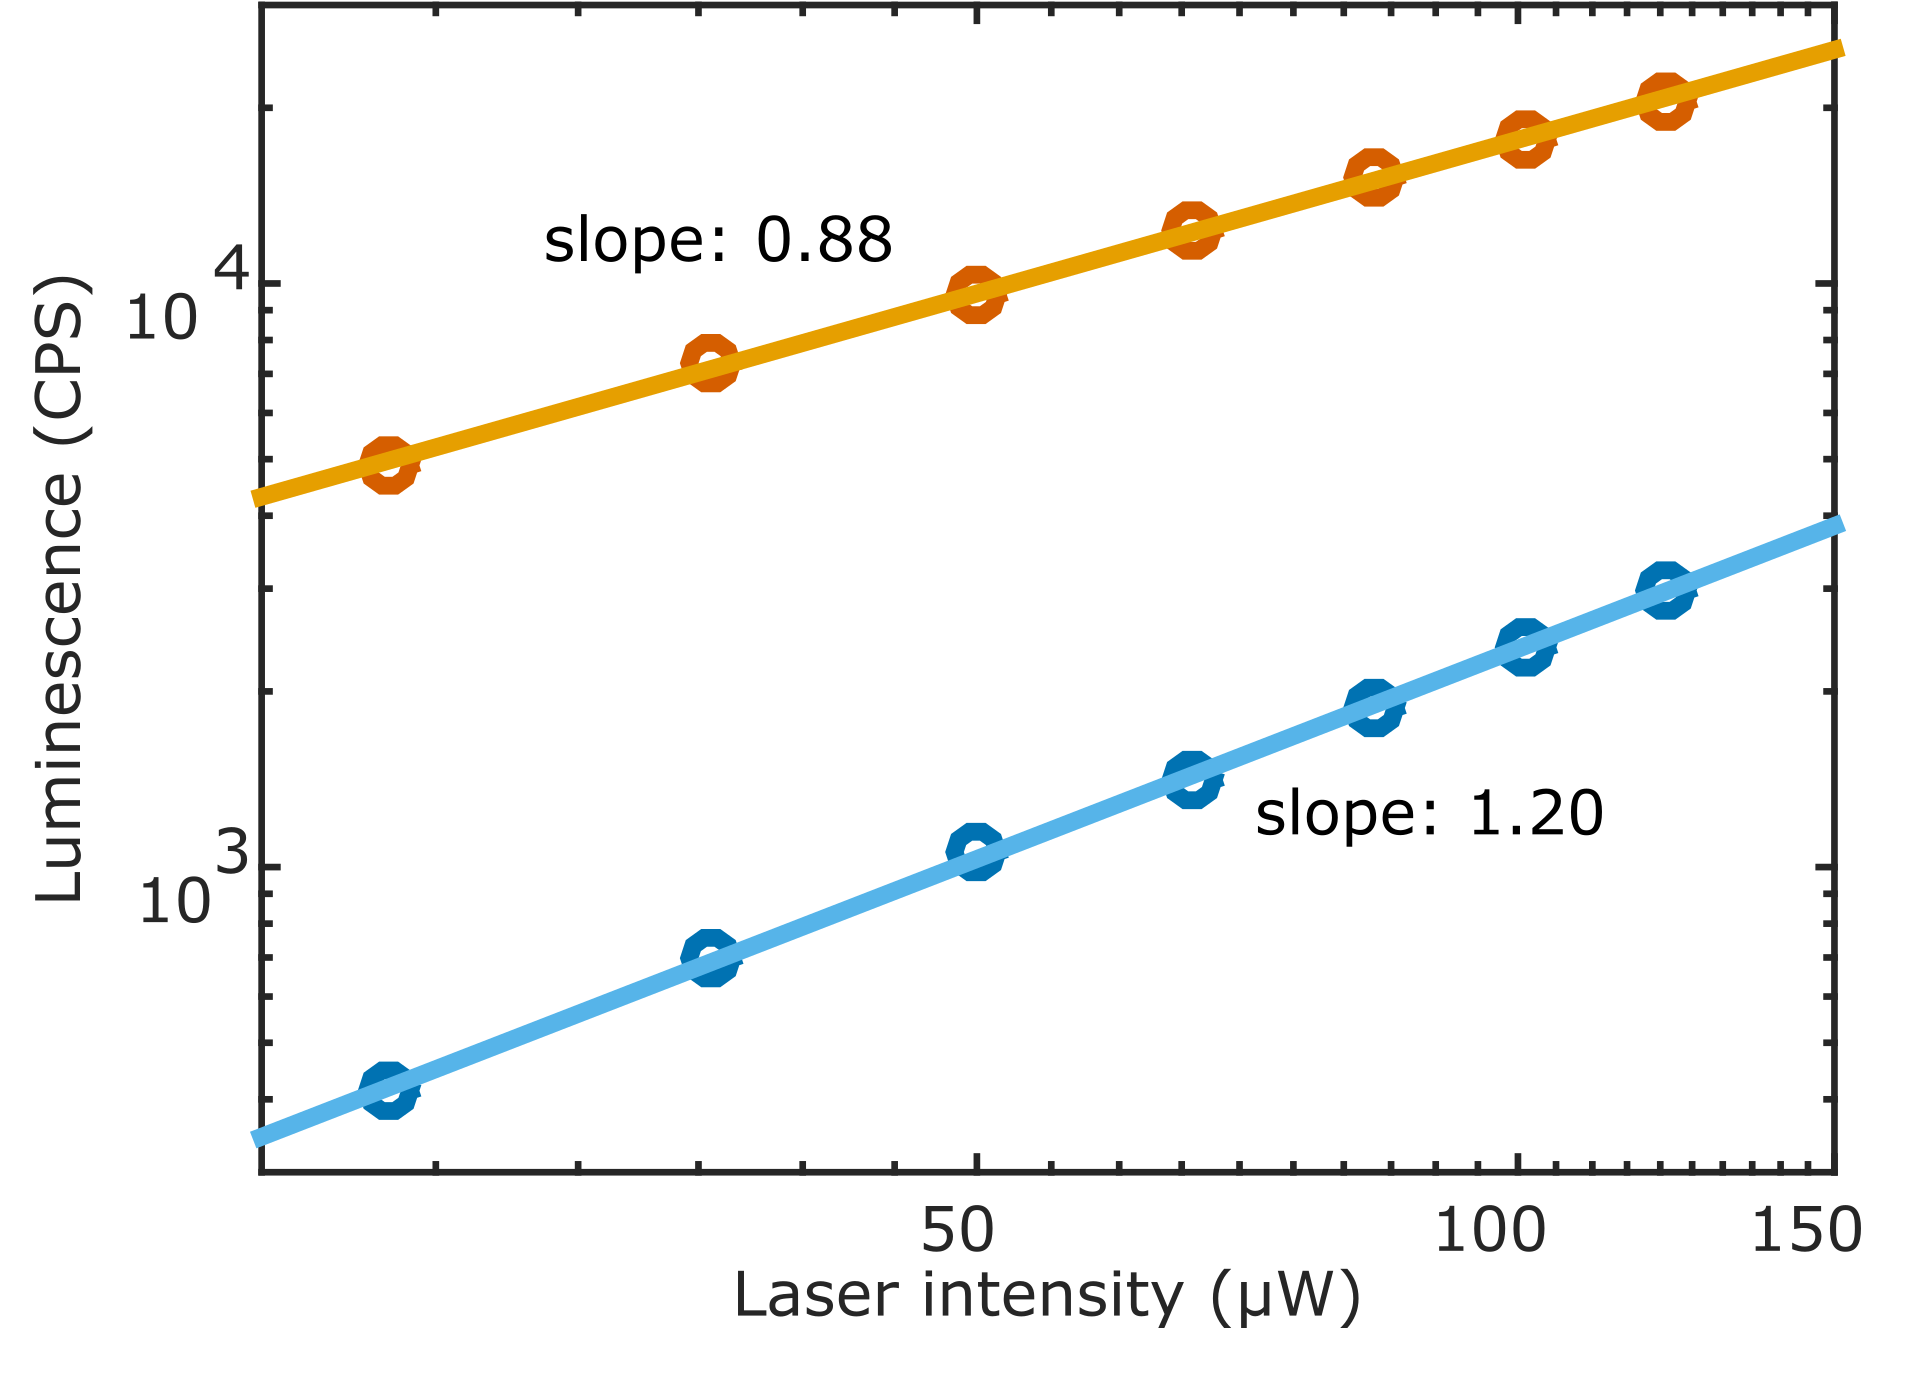
\includegraphics[width=0.45\textwidth]{Figures/Supplementary/03_AS_S_in_Log/03_AS_S_in_Log.png}
\caption{Stokes and anti-Stokes integrated emission as a function of excitation power. The
linear fit in logarithmic scale has a slope of $0.88$ and $1.20$ respectively,
confirming the 1-photon nature of both kinds of emission.}
	\label{fig:Log_Plot}
\end{figure}

Figure \ref{fig:Log_Plot} shows the intensity of the Stokes (red) and
anti-Stokes (blue) emission for several excitation powers. In both cases the
linear fit in logarithmic scale has a slope close to $1$, being $0.88$ for the
Stokes and $1.20$ for the anti-Stokes, confirming that both types of emission
are single-photon processes. 
The anti-Stokes band has a higher slope due to dependence on $T$ of the 
anti-Stokes emission and to nanorod heating at higher power:
 the higher the power, the higher the temperature of the particle and the 
higher the anti-Stokes signal is. This behavior is independent of the plasmon
resonance position. It is important to note that the excitation intensity cannot
be increased much beyond what is shown because nanorods would start reshaping
towards more spherical shapes at higher laser powers.



\section{Gold Nanorod temperature numerical calculations} \label{sec:temp-calc}

\begin{figure}[htp] \centering
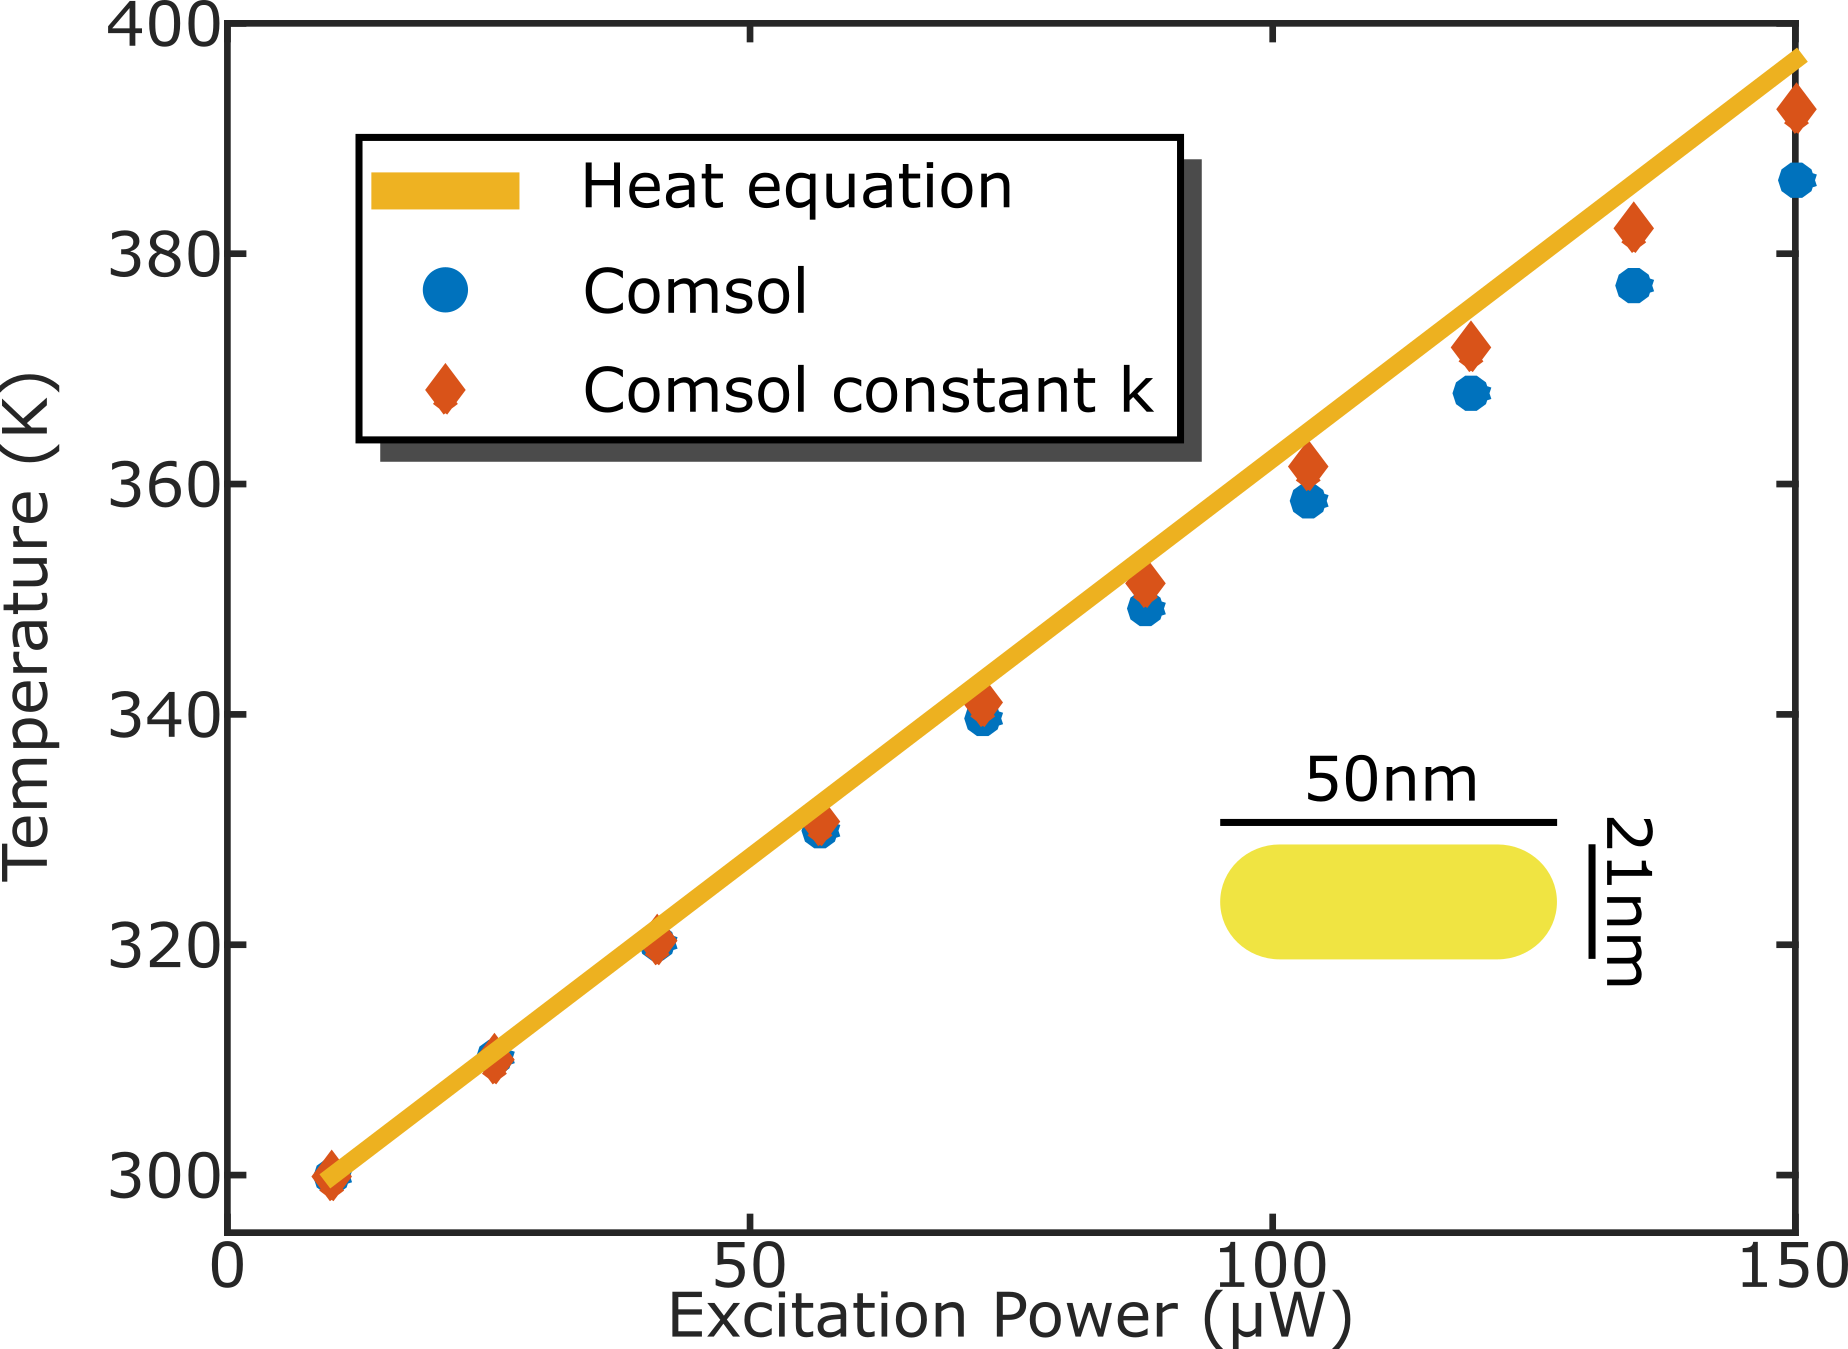
\includegraphics[width=0.5\textwidth]{Figures/Supplementary/04_Compare_Comsol/04_Compare_Comsol.png}
\caption{\textbf{Gold nanorod temperature calculation for different excitation powers.}
Calculated temperature for a nanosphere (full line) and 
for a $21\,\nm\times 50\,\nm$ nanorod (dots) under different excitation intensities. 
The dots are numerically calculated values using COMSOL Multiphysics commercial software. 
The blue dots where obtained with the temperature-dependent heat conductivity of water 
and the red diamonds with a constant value of $0.61 \W(\m\cdot\K)^{-1}$ .}
	\label{fig:Compare-Comsol}
\end{figure}

Throughout the main text the temperature measured with the anti-Stokes emission
is compared to the calculated temperature using the heat diffusion
equation. For spheres in an homogeneous water environment and assuming an infinite
thermal conductivity for the metal, the temperature increase is given by

\begin{equation}
	\Delta \textrm{T}(P) = \frac{P}{4\pi k_{\textrm{water}} R}
\end{equation}

\noindent where $P$ is the dissipated power, $k_{\textrm{water}}$ is the heat
conductivity of water and $R$ is the radius of the particle.\cite{Baffou2013} 
The dissipated power can be
easily derived from the cross section of the particle at a given wavelength and
the intensity of the focused laser beam. For nanorods we assumed an
equivalent sphere with radius such that the total rod area is preserved.

Figure \ref{fig:Compare-Comsol} shows the difference between the results from
the sphere (full line) and a finite element method calculation
(dots) for a nanorod of length $50\nm$ and diameter $21\nm$. The cross section
and dissipated power were kept the same. The blue dots are the results given
by using the built-in material properties of water, i.e. a thermal conductivity
that depends on temperature. The red diamonds are the results when the thermal
conductivity is fixed to $0.61 \W(\m\cdot\K)^{-1}$. The difference is
accentuated at higher temperatures.

%\section{Anti-stokes luminescence form nanospheres}

 %\begin{figure}[tp] \centering
 %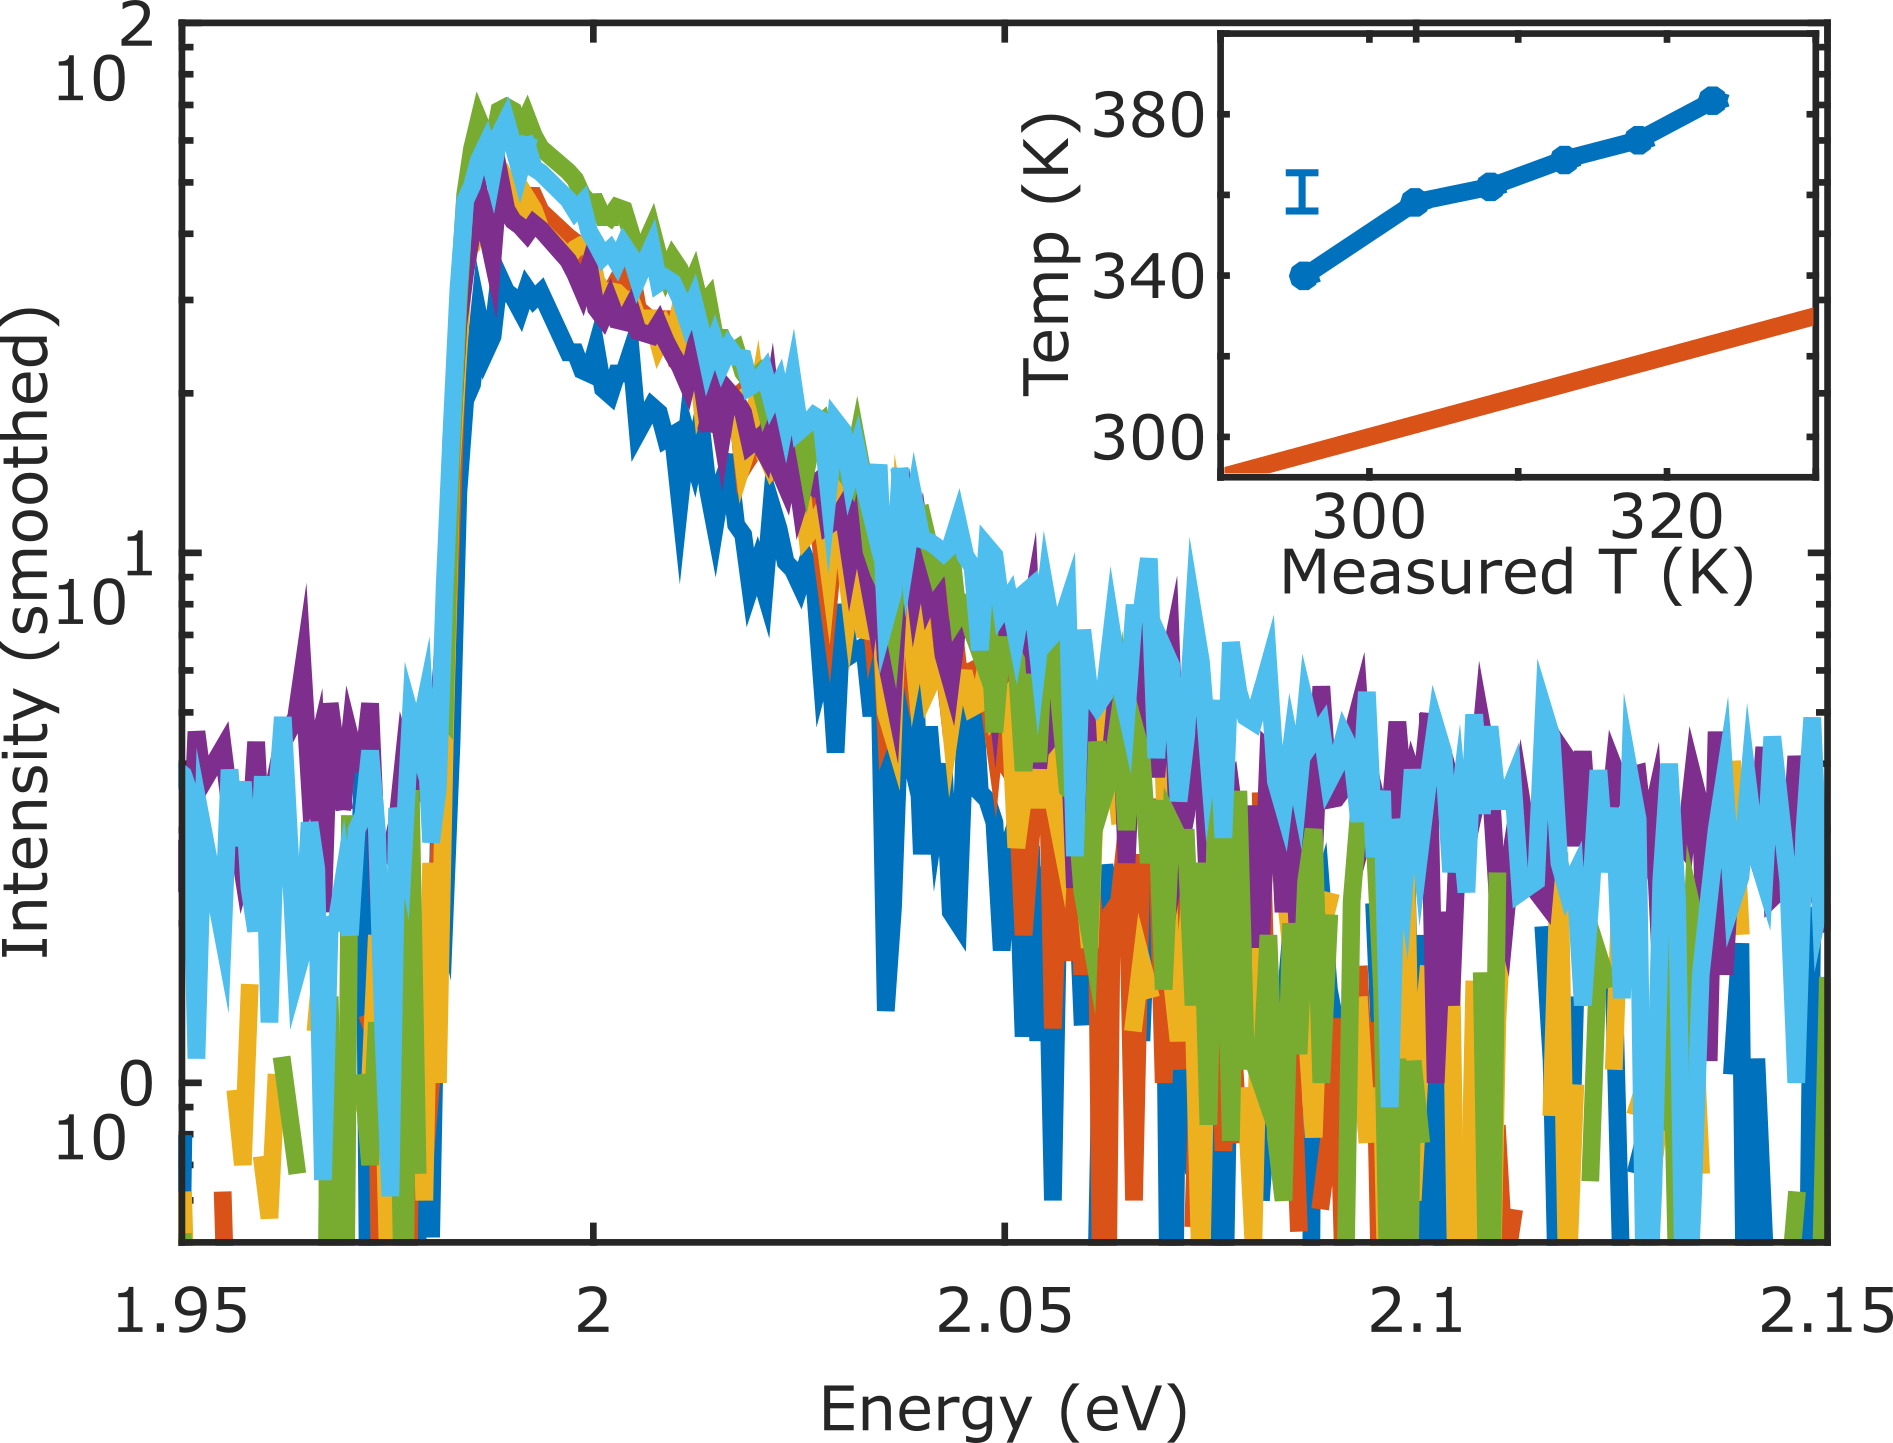
\includegraphics[width=80mm]{Figures/04_Extracted_Temp/04_extracted_temp.png}
 %\caption{Temperature of a single nanorod under the same $633\nm$
 %excitation conditions, but at different medium temperatures. }
 	%\label{fig:AS-temps-rods}
 %\end{figure}
 %
 %It is also possible to keep the excitation intensity constant and to vary the
 %temperature of the surrounding medium. Figure \ref{fig:AS-temps-rods} shows the
 %extracted temperature from the fitting with equation \ref{eqn:fitting} as a
 %function of the temperature of the medium. The red line is showing the water
 %temperature and acts as a guide to the eye. The Figure clearly shows an increase
 %in the extracted temperature while increasing the temperature of the flow cell.
 %The range of explored temperatures was from $296\K$ to $320\K$. This range is
 %enough to observe a change in the anti-Stokes emission spectrum. At higher
 %temperatures the stability of the setup plays a crucial role in maintaining the
 %particle in focus during the spectra acquisition time. Longer exposure times and
 %therefore lower excitation intensities can be employed if particles are actively
 %maintained in focus.
 
 %Particles that can withstand higher excitation powers and that have a
 %well-defined plasmon resonance are of great interest, because they would allow
 %to employ a single wavelength and also to reduce the exposure times to record
 %the spectra. A well defined plasmon resonance also lowers the uncertainties
 %associated with the initial lorentzian fit needed for the term $I_\textrm{SPR}$
 %in equation \ref{eqn:fitting}. In principle gold nanospheres fulfill these
 %requirements. They are known to withstand much higher excitation powers without
 %reshaping nor melting\cite{Hou2015}. Moreover the plasmon resonance of spheres
 %shifts only slightly with radius, therefore it is possible to predict it using
 %Mie theory and to eliminate the need of a second laser beam. Sphere samples
 %however always show a shape distribution that cannot be neglected\cite{Lee2013}
 %and that induces deviations of the observed resonance from Mie's model.
 %
 %\begin{figure}[tp] \centering
 %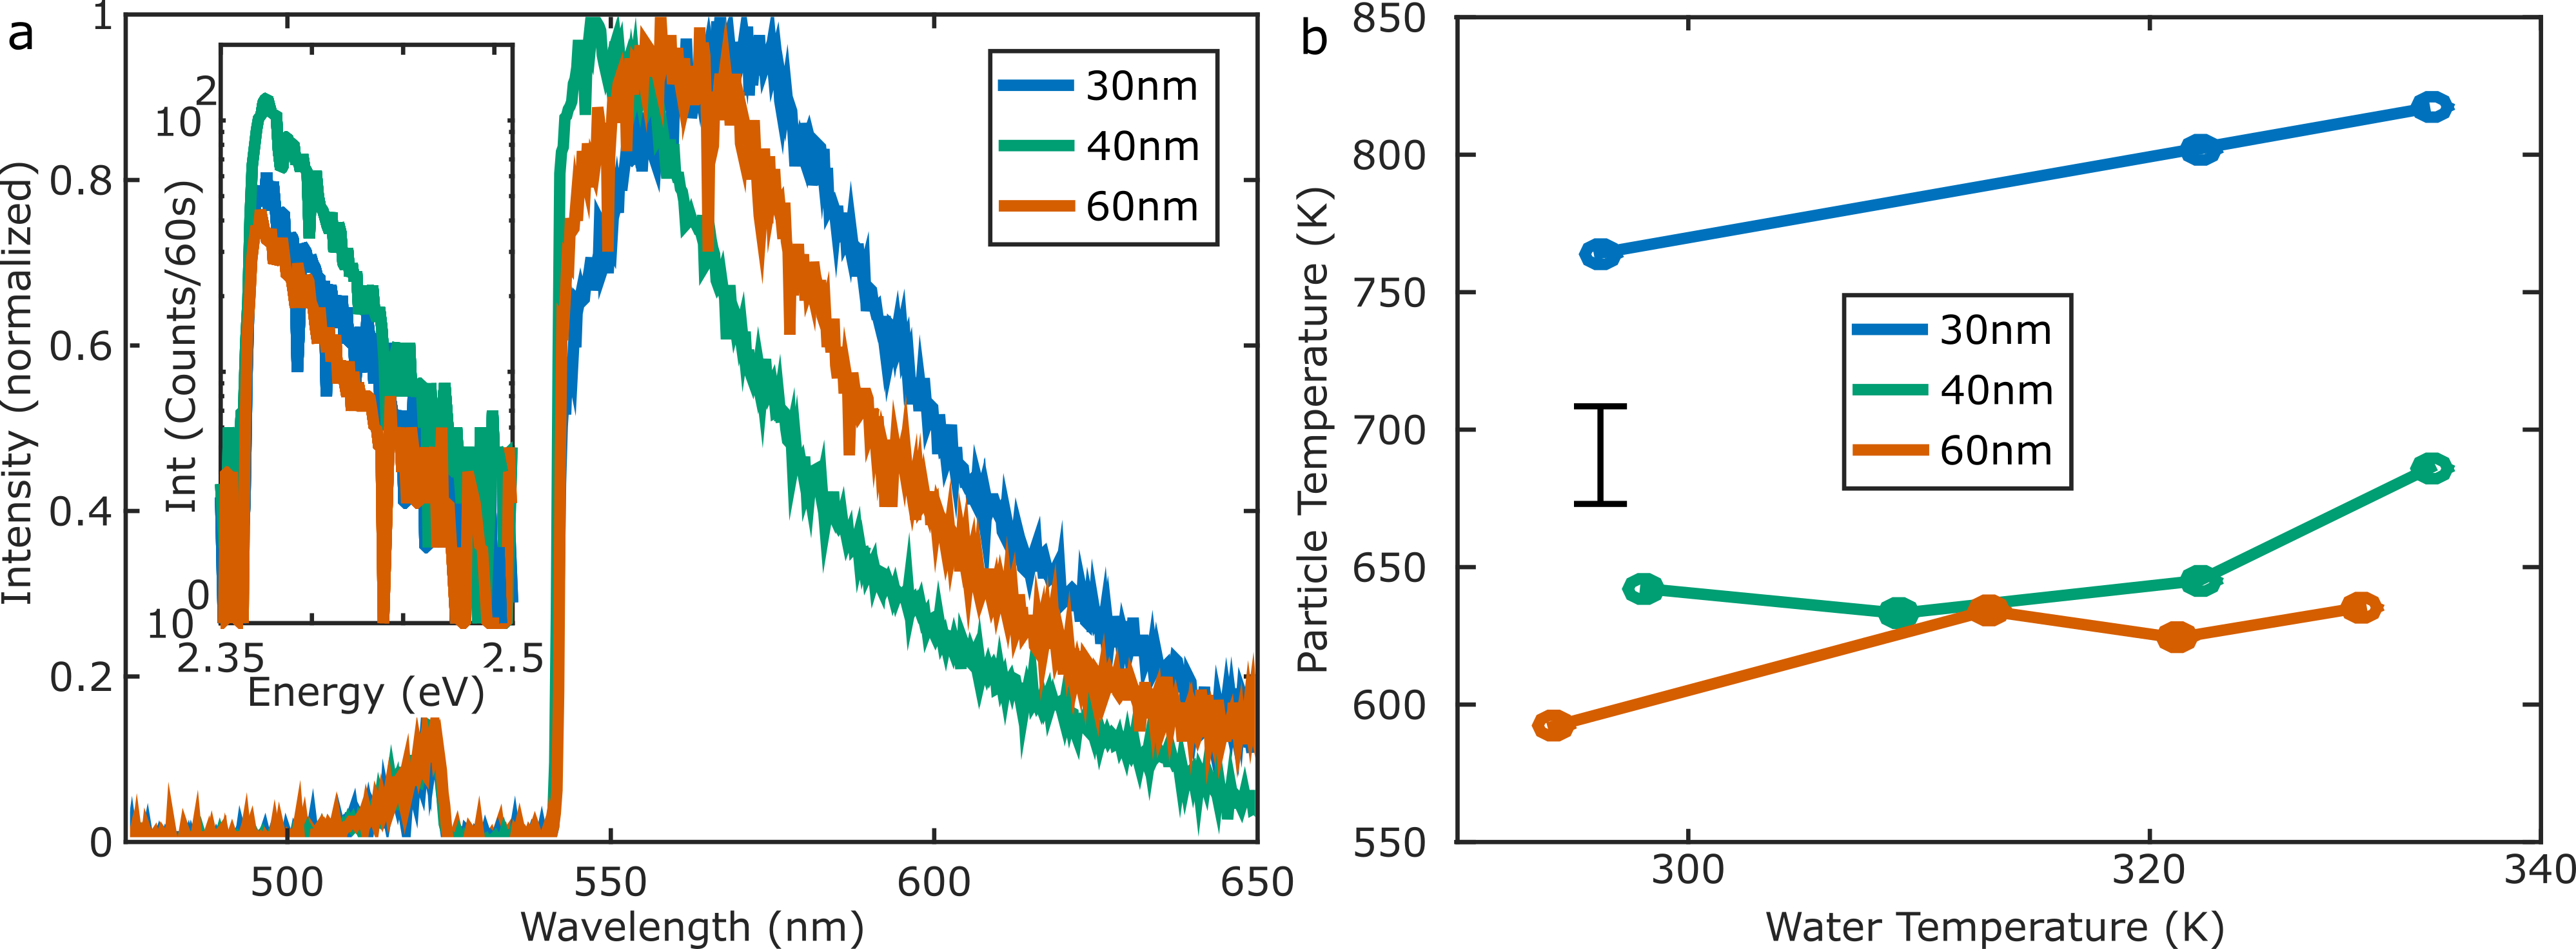
\includegraphics[width=85.2mm]{Figures/07_Spheres/07_spheres.png}
 %\caption{Normalized luminescence spectra of spheres with diameters of $60\nm$,
 %$40\nm$ and $30\nm$ under $532\nm$ excitation. The inset shows the detail of the anti-Stokes emission without normalization.
 %The excitation powers for the three particles were $1.2\mW$, $2.0\mW$ and
 %$3.6\mW$ respectively.}
 	%\label{fig:spheres}
 %\end{figure}
 %
 %Figure \ref{fig:spheres} shows the normalized luminescence spectra of three
 %nanospheres of diameters $60\nm$, $40\nm$ and $30\nm$ under $532\nm$ excitation.
 %As for the nanorods, two very distinctive parts of the spectrum are
 %distinguishable, the Stokes spectrum at longer wavelengths and the anti-Stokes
 %spectrum at shorter ones. From Mie theory we would have expected a blue
 %shift of the resonance with decreasing radius of the particles; however the
 %$30\nm$ sphere seems to be the most red-shifted. This is most likely due to small anisotropies of the
 %particles, giving rise to slightly different plasmon resonances. The inset in
 %Fig.\ref{fig:spheres} shows a detail of the anti-Stokes emission for the three
 %spheres without any further normalization. It has to be pointed out, however,
 %that the excitation intensities were $1.2\mW$, $2.0\mW$ and $3.6\mW$ to
 %compensate for the lower cross sections of the smaller particles.
 %
 %Spheres not only have a smaller cross section than nanorods of the same volume,
 %but their quantum yield is also one order of magnitude lower than that of
 %rods\cite{Yorulmaz2012}. The weaker emission from these particles can be
 %compensated by increasing the excitation power. The maximum power that can be
 %employed is given by either reaching the melting temperature of gold or by
 %inducing a phase transition of the surrounding liquid. The first would induce an
 %irreversible change in shape of the particles\cite{Zijlstra2009a} the latter
 %would induce a change in the refractive index of the medium and therefore would
 %induce a shift in the plasmon resonance\cite{Hou2015}.
 %
 %\begin{figure}[tp] \centering
 %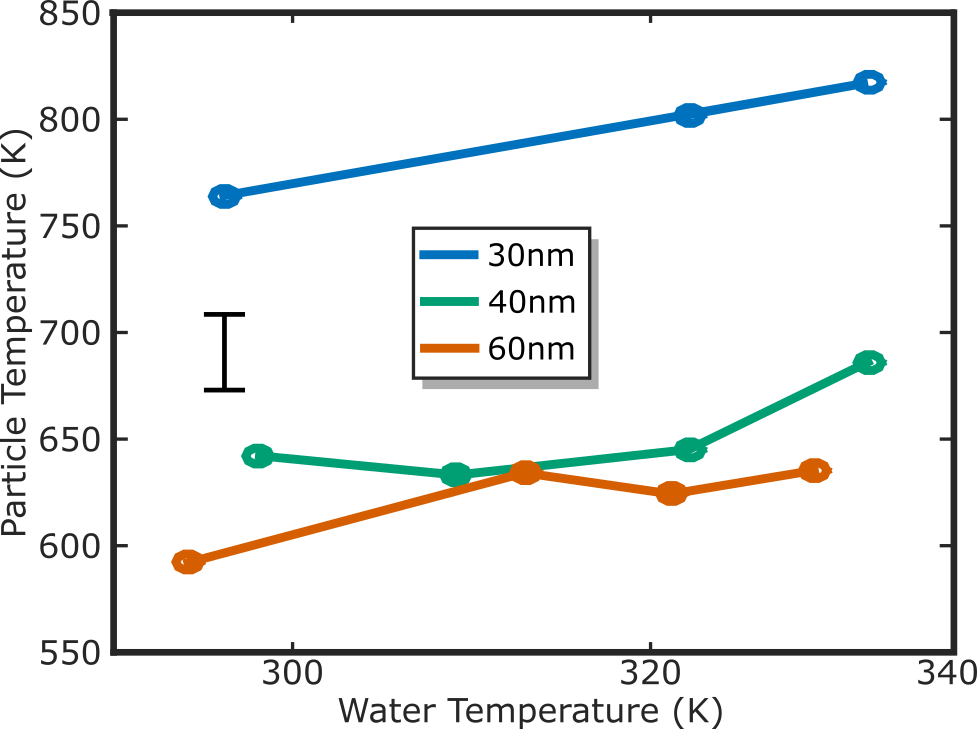
\includegraphics[width=82.7mm]{Figures/07_Spheres/07_spheres_02.png}
 %\caption{Extracted temperature from the same particles as in fig.
 %\ref{fig:spheres} at different medium temperatures. }
 	%\label{fig:spheres_temp}
 %\end{figure}
 %
 %Figure \ref{fig:spheres_temp} shows the extracted temperature of the three
 %particles while increasing the medium temperature. It is possible to see that
 %the small $30\nm$ diameter sphere is $150\K$ hotter than both the $40\nm$ and
 %$60\nm$. The three curves show an increasing trend, but in this case the
 %variation of medium temperature amounts to less than $5\%$ the temperature of
 %the particles. The extracted temperature is several tens of degrees above what
 %would be expected from the heat equation, considering the absorption cross
 %section given by Mie theory. The reason for the discrepancies between the
 %measured values and the expected values can be accounted for by the computation
 %of the plasmon resonance term $I_\textrm{SPR}$ in eqn. \ref{eqn:fitting}.
 %
 %As explained earlier for nanorods, the fitting of the anti-Stokes emission is
 %highly sensitive to the plasmon position relative to the laser employed. In the
 %case of nanospheres, the resonance is slightly shifted to the red from the
 %$532\nm$ laser. Small errors in the determination of the plasmon resonance will
 %generate larger errors in the temperature extracted. The differences between the
 %plasmon observed in fig. \ref{fig:spheres} and the results of Mie scattering
 %calculations most likely are due to particles that are not spherical. If this
 %was the case, the calculated cross section and plasmon resonance will not
 %coincide with the particles under study, leading to larger errors.
 %
 %The use of spheres would be beneficial for some applications that require higher
 %excitation powers or smaller particles. The intrinsic heterogeneity of the
 %samples, however, prevents the use of a single wavelength for the measurements.
 %Ideally, white light scattering of single gold nanospheres would provide the
 %information on the plasmon resonance needed for the correct fitting of the
 %anti-Stokes emission. 


\bibliography{anti_stokes}
\end{document}
